\section{Date: 2026-08-09}
\noindent \textbf{Series ID: N3305C0A144NBEA} 

\noindent This series is titled Net corporate dividends: Domestic industries: Forestry, fishing, and related activities and has a frequency of Annual. The units are Millions of Dollars and the seasonal adjustment is Not Seasonally Adjusted.The observation start date is 1998-01-01 and the observation end date is 2022-01-01.The popularity of this series is 1. \\ 

\noindent \textbf{Series ID: CUUSD000SA0L5} 

\noindent This series is titled Consumer Price Index for All Urban Consumers: All Items Less Medical Care in Size Class D (DISCONTINUED) and has a frequency of Semiannual. The units are Index 1982-1984=100 and the seasonal adjustment is Not Seasonally Adjusted.The observation start date is 1984-01-01 and the observation end date is 2017-07-01.The popularity of this series is 1. \\ 

\subsection{Raw Regression}
\noindent Regresses the two series against each other directly. A significant result here can come just as easily from both series sharing a long-run trend as from any real relationship.

\begin{center}
\begin{tabular}{lclc}
\toprule
\textbf{Dep. Variable:}               & value\_fred\_CUUSD000SA0L5 & \textbf{  R-squared:         } &     0.845   \\
\textbf{Model:}                       &            OLS             & \textbf{  Adj. R-squared:    } &     0.837   \\
\textbf{Method:}                      &       Least Squares        & \textbf{  F-statistic:       } &     98.42   \\
\textbf{Date:}                        &      Sun, 09 Aug 2026      & \textbf{  Prob (F-statistic):} &  1.01e-08   \\
\textbf{Time:}                        &          12:22:58          & \textbf{  Log-Likelihood:    } &   -73.000   \\
\textbf{No. Observations:}            &               20           & \textbf{  AIC:               } &     150.0   \\
\textbf{Df Residuals:}                &               18           & \textbf{  BIC:               } &     152.0   \\
\textbf{Df Model:}                    &                1           & \textbf{                     } &             \\
\textbf{Covariance Type:}             &         nonrobust          & \textbf{                     } &             \\
\bottomrule
\end{tabular}
\begin{tabular}{lcccccc}
                                      & \textbf{coef} & \textbf{std err} & \textbf{t} & \textbf{P$> |$t$|$} & \textbf{[0.025} & \textbf{0.975]}  \\
\midrule
\textbf{const}                        &     130.2316  &        6.409     &    20.322  &         0.000        &      116.768    &      143.695     \\
\textbf{value\_fred\_N3305C0A144NBEA} &       0.0385  &        0.004     &     9.921  &         0.000        &        0.030    &        0.047     \\
\bottomrule
\end{tabular}
\begin{tabular}{lclc}
\textbf{Omnibus:}       &  0.145 & \textbf{  Durbin-Watson:     } &    1.621  \\
\textbf{Prob(Omnibus):} &  0.930 & \textbf{  Jarque-Bera (JB):  } &    0.251  \\
\textbf{Skew:}          & -0.170 & \textbf{  Prob(JB):          } &    0.882  \\
\textbf{Kurtosis:}      &  2.569 & \textbf{  Cond. No.          } & 4.82e+03  \\
\bottomrule
\end{tabular}
%\caption{OLS Regression Results}
\end{center}

Notes: \newline
 [1] Standard Errors assume that the covariance matrix of the errors is correctly specified. \newline
 [2] The condition number is large, 4.82e+03. This might indicate that there are \newline
 strong multicollinearity or other numerical problems.

\begin{figure}
\centering
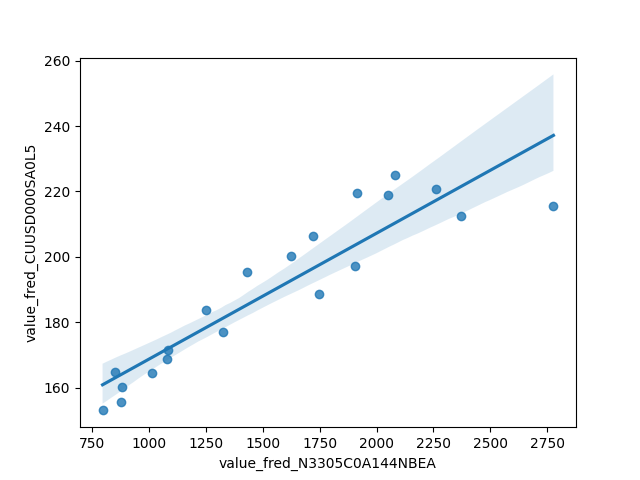
\includegraphics[scale = 0.9]{plots/plot_2026-08-09.png}
\caption{Raw Regression Plot for 2026-08-09}
\end{figure}
\newpage
\subsection{Detrended Regression}
\noindent Regresses the residuals of each series after removing its own linear time trend, so a shared trend can no longer drive the result on its own. A relationship that stays significant here is better evidence of a genuine link between the two series.

\begin{center}
\begin{tabular}{lclc}
\toprule
\textbf{Dep. Variable:}                          & value\_fred\_CUUSD000SA0L5\_detrended & \textbf{  R-squared:         } &     0.364   \\
\textbf{Model:}                                  &                  OLS                  & \textbf{  Adj. R-squared:    } &     0.328   \\
\textbf{Method:}                                 &             Least Squares             & \textbf{  F-statistic:       } &     10.29   \\
\textbf{Date:}                                   &            Sun, 09 Aug 2026           & \textbf{  Prob (F-statistic):} &  0.00487    \\
\textbf{Time:}                                   &                12:22:58               & \textbf{  Log-Likelihood:    } &   -43.796   \\
\textbf{No. Observations:}                       &                     20                & \textbf{  AIC:               } &     91.59   \\
\textbf{Df Residuals:}                           &                     18                & \textbf{  BIC:               } &     93.58   \\
\textbf{Df Model:}                               &                      1                & \textbf{                     } &             \\
\textbf{Covariance Type:}                        &               nonrobust               & \textbf{                     } &             \\
\bottomrule
\end{tabular}
\begin{tabular}{lcccccc}
                                                 & \textbf{coef} & \textbf{std err} & \textbf{t} & \textbf{P$> |$t$|$} & \textbf{[0.025} & \textbf{0.975]}  \\
\midrule
\textbf{const}                                   &   -3.377e-12  &        0.510     & -6.63e-12  &         1.000        &       -1.070    &        1.070     \\
\textbf{value\_fred\_N3305C0A144NBEA\_detrended} &       0.0065  &        0.002     &     3.208  &         0.005        &        0.002    &        0.011     \\
\bottomrule
\end{tabular}
\begin{tabular}{lclc}
\textbf{Omnibus:}       &  0.582 & \textbf{  Durbin-Watson:     } &    1.515  \\
\textbf{Prob(Omnibus):} &  0.747 & \textbf{  Jarque-Bera (JB):  } &    0.620  \\
\textbf{Skew:}          &  0.127 & \textbf{  Prob(JB):          } &    0.734  \\
\textbf{Kurtosis:}      &  2.176 & \textbf{  Cond. No.          } &     253.  \\
\bottomrule
\end{tabular}
%\caption{OLS Regression Results}
\end{center}

Notes: \newline
 [1] Standard Errors assume that the covariance matrix of the errors is correctly specified.

\begin{figure}
\centering
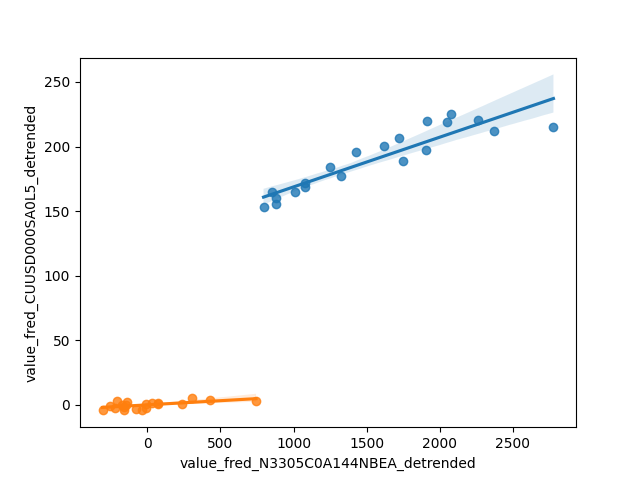
\includegraphics[scale = 0.9]{plots/plot_2026-08-09_detrended.png}
\caption{Detrended Regression Plot for 2026-08-09}
\end{figure}
\newpage
